%----------------------------------------------------------------------------------------
%	KENAN FIRMANSYAH - GENERAL SOFTWARE ENGINEER VARIANT
%----------------------------------------------------------------------------------------

\documentclass[11pt,a4paper]{article}

\usepackage[utf8]{inputenc}
\usepackage[T1]{fontenc}
\usepackage{lmodern}
\usepackage[margin=0cm]{geometry}
\usepackage{hyperref}
\usepackage{fontawesome5}
\usepackage{xcolor}
\usepackage{tikz}
\usepackage{graphicx}
\usepackage{enumitem}
\usepackage{parskip}
\usepackage{multicol}
\usepackage{fancyhdr}
\usepackage{calc}

\definecolor{sidebar}{RGB}{245, 245, 245}
\definecolor{mainbg}{RGB}{255, 255, 255}
\definecolor{accent}{RGB}{180, 150, 100}
\definecolor{darktext}{RGB}{40, 40, 40}
\definecolor{lighttext}{RGB}{100, 100, 100}

\hypersetup{
    colorlinks=true,
    linkcolor=darktext,
    urlcolor=accent,
    pdftitle={Kenan Firmansyah - Software Engineer Resume},
    pdfauthor={Kenan Firmansyah}
}

\pagestyle{empty}
\setlength{\parindent}{0pt}

\newcommand{\sidesection}[1]{%
    {\large\bfseries\MakeUppercase{#1}}\\[6pt]%
}

\newcommand{\mainsection}[1]{%
    {\large\bfseries\MakeUppercase{#1}}\\[8pt]%
}

\newcommand{\jobentry}[2]{%
    \textbf{#1}\\
    {\small\color{lighttext}#2}\\[4pt]%
}

\begin{document}

\begin{tikzpicture}[remember picture, overlay]
    \fill[sidebar] (current page.north west) rectangle ([xshift=6.5cm]current page.south west);
    \fill[mainbg] ([xshift=6.5cm]current page.north west) rectangle (current page.south east);
    \fill[accent] ([xshift=6.5cm, yshift=-1cm]current page.north west) rectangle ([yshift=-1.05cm]current page.north east);
\end{tikzpicture}

\begin{minipage}[t]{6cm}
\vspace{0.8cm}
\hspace{0.5cm}
\begin{minipage}[t]{5.5cm}

\begin{center}
\begin{tikzpicture}
    \clip (0,0) rectangle (4.5cm, 4.5cm);
    \node[anchor=center] at (2.25cm, 2.25cm) {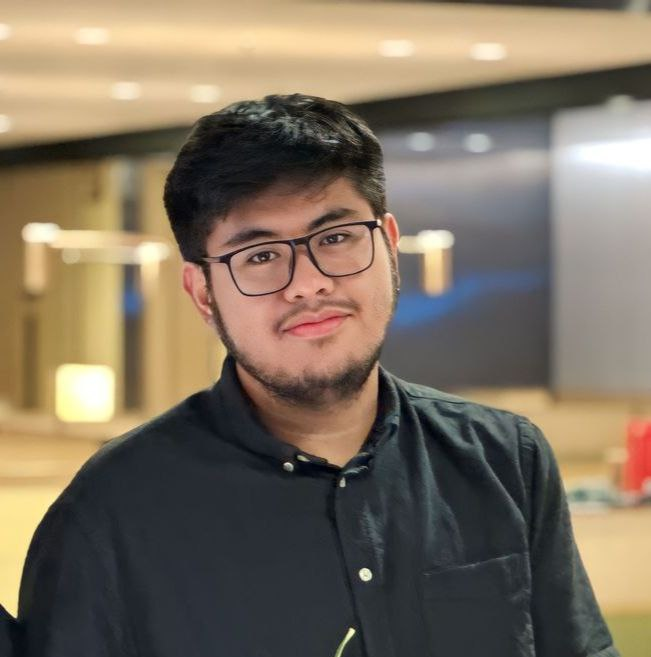
\includegraphics[width=4.5cm]{CV_ProfilePic.jpg}};
\end{tikzpicture}
\end{center}

\vspace{0.8cm}

\sidesection{Education}

\textbf{Bachelor of Computer Engineering, Major in Game Technology}\\[4pt]
{\small Electronic Engineering Polytechnic Institute of Surabaya (2020 - 2024)\\
GPA 3.67 (Cumlaude)}

\vspace{0.8cm}

\sidesection{Technical Skills}

\begin{itemize}[leftmargin=*, nosep, itemsep=4pt]
    \item Languages: Python, C++, C\#, Swift
    \item Engines: Unreal (Blueprint + C++), Unity
    \item Mobile: SwiftUI, UIKit (iOS)
    \item Data: NumPy, Selenium, Tableau
    \item AI/ML: Reinforcement Learning, Fuzzy Logic
\end{itemize}

\vspace{0.8cm}

\sidesection{Contact}

\faIcon{linkedin} \href{https://linkedin.com/in/kenanfirmansyah}{Kenan Firmansyah}\\[6pt]
\faIcon{github} \href{https://github.com/Kenanfir}{Kenanfir}\\[6pt]
\faIcon{globe} \href{https://nandev.dev}{nandev.dev}\\[6pt]
\faIcon{phone} +6285175447540\\[6pt]
\faIcon{envelope} realkenanfir@gmail.com\\[10pt]

{\small\color{lighttext}Kalijudan, Mulyorejo, Surabaya, Jawa Timur 60114}\\[6pt]

{\small\color{lighttext}Holland Village Jakarta, Cemp. Putih, Jakarta Pusat, DKI Jakarta 10510}

\end{minipage}
\end{minipage}%
%
\begin{minipage}[t]{14cm}
\vspace{0.5cm}
\hspace{0.8cm}
\begin{minipage}[t]{12.5cm}

{\Huge\bfseries\MakeUppercase{Kenan Firmansyah}}\\[6pt]
{\large\bfseries SOFTWARE ENGINEER}\\[12pt]

{\small Software engineer with experience across game development, mobile, applied AI/ML research, and data engineering. Five peer-reviewed publications and multiple shipped products on the iOS and Mac App Stores.}

\vspace{0.6cm}

\mainsection{Experience}

\jobentry{Game Developer}{Agate | 2026 Feb - 2026 May}
\begin{itemize}[leftmargin=*, nosep, itemsep=2pt, topsep=2pt]
    \item Software engineering on an unannounced commercial project at one of Indonesia's largest game studios.
\end{itemize}

\vspace{0.3cm}

\jobentry{Apple Developer Academy @ BINUS (Alum)}{2025 Feb - 2025 Dec, Bali}
\begin{itemize}[leftmargin=*, nosep, itemsep=2pt, topsep=2pt]
    \item 10-month intensive in Apple-platform development; design thinking, user research, prototyping, iterative testing.
    \item \textbf{Won 1st Place at iPlay ADA Game Jam 2025} (System \& AI Programmer).
\end{itemize}

\vspace{0.3cm}

\jobentry{Lead Developer (Unreal Engine)}{Starpixel Studios | 2024 Oct - 2025 April}
\begin{itemize}[leftmargin=*, nosep, itemsep=2pt, topsep=2pt]
    \item Led a multiplayer horror project; gameplay systems, networking, Blueprint with C++ for hot paths.
    \item Weekly builds, bug triage, internal technical documentation.
\end{itemize}

\vspace{0.3cm}

\jobentry{Data Scientist (Intern)}{PT. eBdesk | 2023, 6 months}
\begin{itemize}[leftmargin=*, nosep, itemsep=2pt, topsep=2pt]
    \item Python pipelines for scraping, analysis, and visualization (Selenium, Gephi, Tableau).
\end{itemize}

\end{minipage}
\end{minipage}

\newpage

\begin{tikzpicture}[remember picture, overlay]
    \fill[accent] (current page.north west) rectangle ([yshift=-0.8cm]current page.north east);
\end{tikzpicture}

\vspace{1.2cm}

\begin{center}
{\large\bfseries\MakeUppercase{Additional Experiences \& Projects}}
\end{center}

\vspace{0.5cm}

\hspace{1cm}
\begin{minipage}[t]{18cm}

\begin{minipage}[t]{0.8cm}
{\Large\bfseries 1}
\end{minipage}%
\begin{minipage}[t]{17cm}
{\large\bfseries SHIPPED PRODUCTS}\\[8pt]

\textbf{Saturated} (Mac App Store, Apple Silicon) — Programmer \& Project Manager, JoyBait Studio (2025 Oct - Dec).\\
\textbf{Milky Ice Jump} (iOS App Store) — Freelance iOS port + ad integration (2025 Oct).\\
\textbf{Apple Developer Academy cohort apps:} Findect, Paid, Tona, Pet Jam, Rantify (Swift / SwiftUI, 2025).

\end{minipage}

\vspace{0.5cm}

\begin{minipage}[t]{0.8cm}
{\Large\bfseries 2}
\end{minipage}%
\begin{minipage}[t]{17cm}
{\large\bfseries SELECTED RESEARCH \& PUBLICATIONS}\\[8pt]

\textbf{Adaptive Radio System Using MetaSounds for Serious VR Game} — IEEE Access (Vol. 13), Nov 2, 2025.\\
\textbf{Dynamic Difficulty Using Q-Learning and Fuzzy Logic} — IEEE Access (Vol. 12), Sep 12, 2024. \emph{+35\% session length}.\\
\textbf{Context-Aware Recommender System for In-Game Radio} — INASS IJIES, Sep 2, 2024. \emph{F1 up to 0.71}.\\
\textbf{Real Time Procedural Audio with MetaSounds} — TCCE 2025.\\
\textbf{Dynamic Day and Night Cycle in a Serious VR Game} — ICVR 2024.

\end{minipage}

\vspace{0.5cm}

\begin{minipage}[t]{0.8cm}
{\Large\bfseries 3}
\end{minipage}%
\begin{minipage}[t]{17cm}
{\large\bfseries OTHER PROJECTS}\\[8pt]

\textbf{Xanthous (Thesis, EEPIS)} — AI-driven VR horror game in Unreal (2023 Feb - 2024 July).\\
\textbf{Game Jams (9+):} Brackeys, GMTK, ScoreSpace, Ryan Laley, Global Game Jam, Garena, Candela, GAMELOFT, IGGI — varied roles across gameplay, AI, and solo development in Unity and Unreal.\\
\textbf{Home Server (Personal, 2023)} — Multi-purpose Proxmox setup (NAS, database, compute) on Linux.\\
\textbf{Indonesia Game Island 2026} — Logistics \& Community Manager for JoyBait Studio booth.

\end{minipage}

\vspace{0.8cm}

\begin{center}
\href{https://nandev.dev}{\bfseries\color{accent}\underline{View More...}}\\[4pt]
{\small nandev.dev}
\end{center}

\end{minipage}

\end{document}
